
\chapter{Introduction}

% In nowadays there are many


Important issue in many NLP appliance is to arrange proper treatment for collocations. What is collocation will be described in 
section \ref{col_def}, but for now assume that it is "habitual recurrent word combinations of everyday language"\cite{ramisch}.
It is essential because multi-word expressions occure very frequently, some researches\footnote{
\textit{The Architecture of the Language Faculty}, Jackendoff R., 1997} shows that they constitute half of the native speakers lexicon.
If some NLP application does not handle MWE properly it will probably generate ungrammatical or unnatural output.
To avoid such situation, dictionaries, that are used in NLP, should include collocations as well. Completion of those dictionaries 
requires significant manual labor, so to facilitate this process programs for automatic extraction of collocations are used.

Thesis describes the process of improving web based system for extraction of collocations called MeWeX. 
At first it introduces the problem of automatic extraction of collocations and introduces the system itself, 
its structure and functioning. Next chapters present all steps which were performed in order to improve quality of the MeWeX.

\section{Definition of collocation}\label{col_def}
Precise defining collocation is not a simple task and this issue was illustrated in \cite{evert} 
\textit{"Even though any two lexicographers would agree that ’once upon a time’, ’hit the road’ and similar idioms are collocations,
they would most certainly disagree on almost anything else."}.
Lexicographers argued over the years on correct defining what collocation is and because of that there is no one fixed definition of collocation  
and in relevant literature we can find many different versions but most of them have one common characteristic, 
collocation is a multiword expression that are syntactically and/or semantically idiomatic. Because this thesis will base on MeWeX system 
it assumes the same definition as in \cite{mgr}, for which purpose MeWeX was created.
\begin{quote}
    Collocation is a multiword specialistic term or noncompositional general term. 
    It may be both continous or not and both in fixed or flexible order.
    % Za wyrażenie wielowyrazowe uznawane są wieloelementowe terminy specjalistyczne oraz
    % niekompozycyjne terminy ogólne. Mogą być one zarówno ciągłe, w szyku przemiennym, jak i
    % ustalonym.
\end{quote}
This definition was motivated by similarity to others definitions used by lexicographers and it fits the needs for creating polish multi-word expressions dictionary. 

\section{Methods for extraction of collocations} \label{extraction_method}
Automatic extraction of collocations is a hard task \cite{ramisch}. First of all precise specification of collocation is required.
Method of extraction is dependent on choosen definition of MWE but also on other factors like language. 
Even having precisly specified all conditions it may be performed in many different ways. 
Usually finding MWE consists of three steps. At first candidates for collocation are extracted from the text using some rules and filters, 
which most often base on grammar of given language. Second step is to evaluate quality of the candidates 
using some association measure or more sophisticated algorithms and sorting it according to obtained values. 
Finally collocations are choosen from generated ranking. Method used in MeWeX is similar to the mentioned above general way, 
more detailed description is included in section \ref{mewex_workflow}.

\section{MeWeX}
MeWeX is a system designed for extraction of collocations created for purposes of \cite{mgr}. It is designed as a set of separate programs 
that preforms consequitive parts of extraction process, but it can be also used as a software library in other projects. 
This design gives huge flexibility, because it allows to run given part many times in different setup, 
or to preprocess large data and save result of every step. This capabilities are very useful in conducting reaserch. 
It is also helpful in natural language processing where often size of data is very large, so possibility 
to preprocess input once and repeating further stages many times with different setup can save a lot of time.

\subsection{Analysis of functional and nonfunctional requirements}
some words about requirements
\\\textbf{Functional requirements}
\begin{itemize}
    \setlength\itemsep{0em}
    \item Filter out tuples using specified by the user filter.
    \item Extract candidates from given corpus using specified set of WCCL operators.
    \item Evaluate quality of tuple using association measure.
    \item Evaluate quality of tuple using aggregated vector of association measures.
    \item Create ranking basing on tuple's score.
    \item Examine coverage of extracted collocations in relations set.
    \item Creates matrix that shows intersection of extracted tuples between relations.
    \item Reduce the number of false candidates from set of all generated tuples.
    \item Evaluate quality of results using specified measure.
    \item Return k-best list from given text file.
\end{itemize}
\textbf{Nonfunctional requirements}
\begin{itemize}
    \setlength\itemsep{0em}
    \item Has possibility to extend set of association measures with new ones.
    \item "Number of measures?"
\end{itemize}

\subsection{Structure of the system}
MeWeX has a lot functionalities, so to preserve clear and maintainable code it has expanded stucture. 
This also simplifie further extensions and modifications of the system. Part of the system structure of more important 
or significant for this thesis components of MeWeX is presented on figure \ref{img_structure} in the form of package diagram.

\begin{figure}[ht]
	\centering
	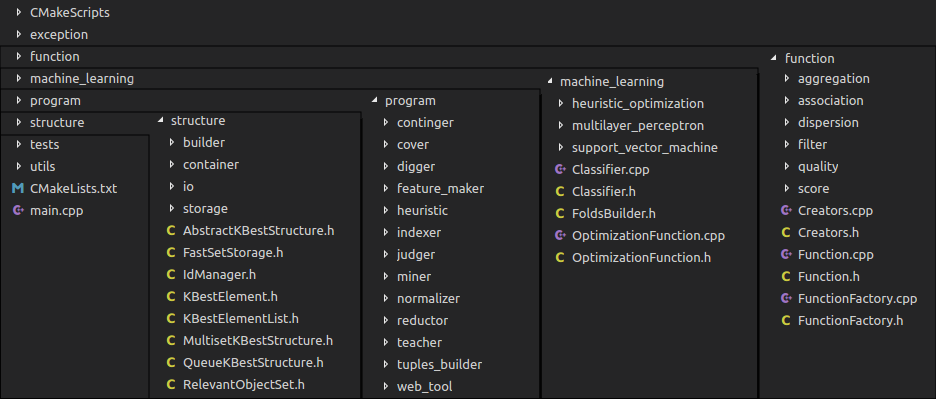
\includegraphics[scale=0.14]{img/mewex_structure.png}
	\caption{Code structure of MeWeX}
	\label{img_structure}
\end{figure}

All functionalities are provided as a set of programs that together creates complete tool for collocation extraction,
verification of the results, tunning weigths, result analysis etc. Below there is a list of all of them together with short description.
\begin{itemize}
    \item \textbf{TuplesBuilder} - Program that reads corpora given as an input and using wccl operators given in input file 
    it creates candidates for collocations.
 
    \item \textbf{Continger} - It creates generators of contingency tables from tuples built by TuplesBuilder.
 
    \item \textbf{Indexer} - This program uses contingency table generators to create set of contingency tables.
 
    \item \textbf{Normalizer} - Program that performs dispersion on contingency tables.
 
    \item \textbf{FeatureMaker} - This program prepares feature vector by evaluating association measures specified at input for each tuple. 
    using output of this program we can train weights for aggregators in reasonable time.
 
    \item \textbf{Heuristic} - It uses given machine learning algorithm to tune weights for association measures. 
    This process is highly adjustable, all parameters for training can be specified in config file.
 
    \item \textbf{Digger} - This program extract collocations basing on given association measures or vector of them. 
    It also provide functionality of extracting encountered forms of collocations.
 
    \item \textbf{Miner} - Program created to perform f-fold, r-round cross validation for choosen association measures or classifiers.
    
    \item \textbf{Cover} - It examines coverage of extracted collocations in relations set. It also creates matrix 
    that shows intersection of extracted tuples between relations. It allows to check how many tuples was assigned to more than one relation 
    and which are the most frequent.
 
    \item \textbf{Judger} - This program evaluates results of extracted collocations. It calculates the percentage of correct MWE.
 
    \item \textbf{Reductor} - This program reduces the number of false candidates from set of all tuples created from the text. 
    Ratio of true to false candidates can be specified in parameter.
 
    \item \textbf{WebTool} - Complex tool that performs whole process of extraction at once, starting from plain text 
    it returns list of extracted collocations.
 
    \item \textbf{Teacher} - Program that can be used for training neural network or support vector machine.
\end{itemize}

\subsection{Workflow of the program} \label{mewex_workflow}
As functionalities of MeWeX are splitted between many separate programs, usually to achive some result several programs must be run in specific order. 
This design, to construct different chains of programs, extends set of possibilities. Some exemplary workflow of the system are described below. 
\\ \\\textbf{Workflow for evaluation of efficiency of methods for extraction of collocations}
\begin{figure}[ht]
	\centering
	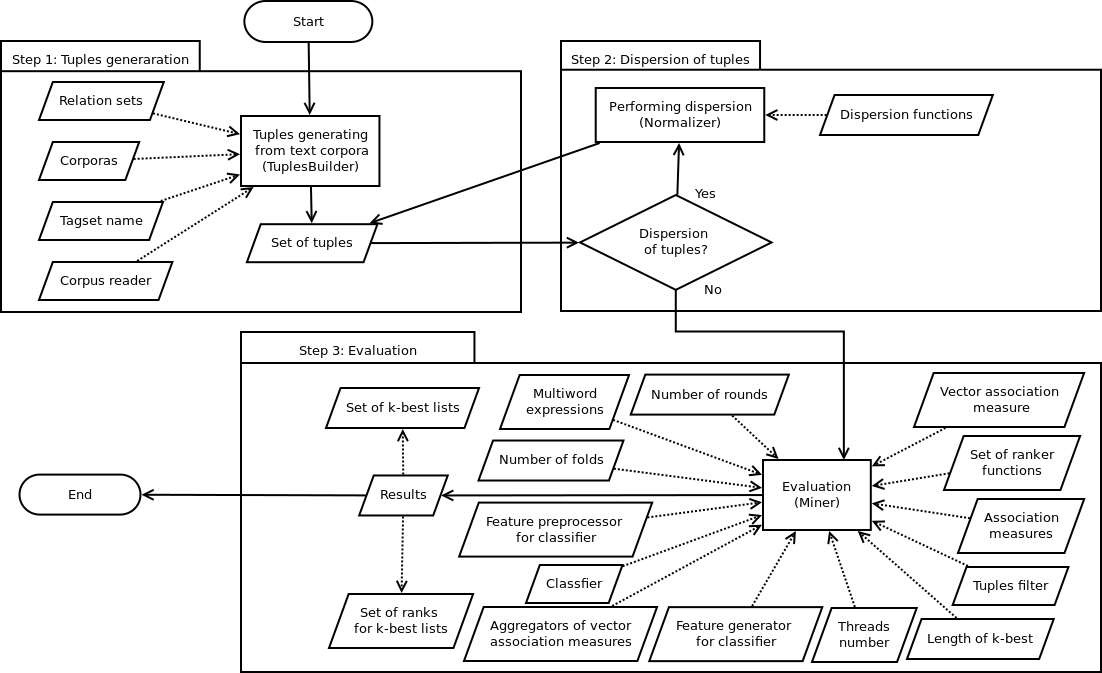
\includegraphics[scale=0.4]{img/mewex_workflow1.png}
	\caption{Examplary workflow}
	\label{img_workflow1}
\end{figure}
\\ Figure \ref{img_workflow1} shows schema of typical path for evaluation of efficiency of given association measure or classifier.
\\ \textbf{Step 1: Tuples generation}\\
First step is to generate tuples from text using WCCL operators, which determine what groups of words are selected for candidates. 
To preform that step program TuplesBuilder is used. It requires list of corpora, corpus reader and name of tagset and 
set of mentioned before wccl operators. Output of this program is CSV file with one tuple per line, consisting information about relation, 
its name, group and size and also all elements of tuple.
\\ \textbf{Step 2: Normalization}\\
Second step is optional and allows modification of information about tuples using one of availble dispersion function. 
It may be useful for processing many corpora of differentiated categories, because it changes frequency distribution of tuples 
favouring less common candidates.
\\ \textbf{Step 3: Evaluation}\\
Final step is to perform f-fold, r-round cross-validation for given dataset. Program accepts as an input many parameters, 
so they are described in table \ref{tbl_workflow1}. After processing it returns 2 sets of files. First type contains k-best list 
of candidates for every fold in every round for every measure and second includes evaluation of those lists. 
Those files should be further analized by the user. 

\begin{table}[t]
    \centering
    % \begin{tabular}{|l|l|}
    \begin{tabular*}{0.9\textwidth}{|l @{\extracolsep{\fill}} l|}
        \hline 
        \textbf{Name of parameter} & \textbf{Description} \\
        \hline
        Tuple storage & Name of the folder with generated tuples \\
        \hline
        Output & Path to the folder were output will be placed \\
        \hline
        Association Measure & Name of association measure to use, \\& this can be specified many times \\
        \hline
        Vector association measure & Text representing vector association measure \\
        \hline
        Aggregator & Aggregator fuction for vector association measure \\
        \hline
        Classifier & Text representing classifier which has to be used \\
        \hline
        Feature generator & Vector association measure which will be used \\& for generating features for classifier \\
        \hline
        Feature preprocessor & Text representing function which has to be used \\& to normalze features for classifier \\
        \hline
        Relevant set & File containing proper MWE, one in line \\
        \hline
        Quality function & Text representing function for evaluation of quality \\& of extracted collocations \\
        \hline
        Tuple filter & Filter that is used to reduce number of tuples \\
        \hline
        Thread number & Maximal number of threads used by program \\
        \hline
        Number of folds & Number of folds for cross-validation \\
        \hline
        Number of rounds & Number of rounds for cross-validation \\
        \hline
    \end{tabular*} 
    \caption{Input parameters for program Miner}
    \label{tbl_workflow1}
\end{table}

\noindent \\\textbf{Workflow for extraction of collocations}
\\ Figure \ref{img_workflow2} shows schema of typical path for extraction of MWEs using given association measure or classifier.
Steps 1 and 2 are identical as in previous example, so they will not be described again.
\begin{figure}[ht]
	\centering
	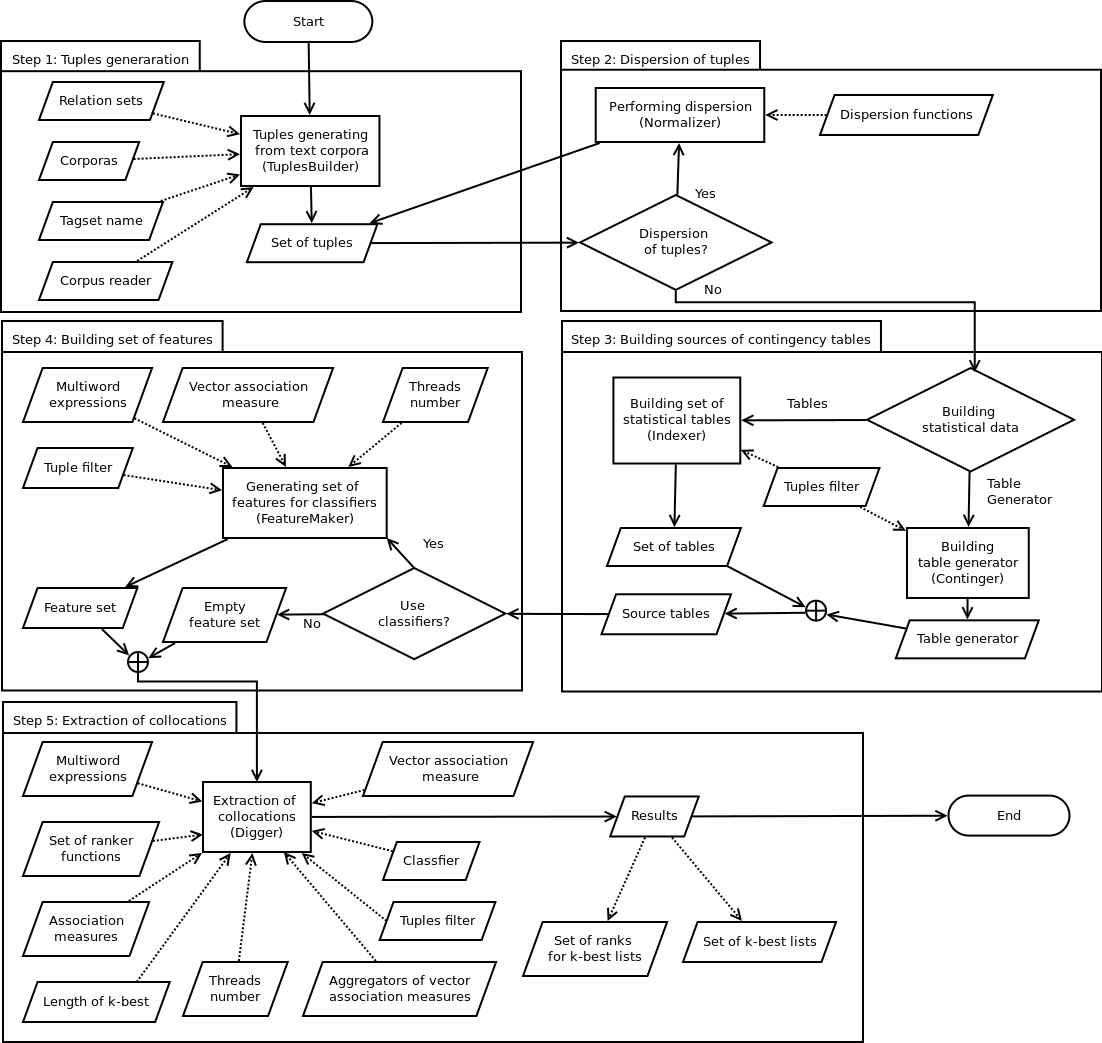
\includegraphics[scale=0.4]{img/mewex_workflow2.png}
	\caption{Examplary workflow}
	\label{img_workflow2}
\end{figure}
\textbf{Step 3: Building contingency table}\\
All measures needs statistical data contained in contingency tables, so they must be generated for further process. 
There are two ways of creating that tables. First is to use Continger, which prepares source of contingency tables, 
this solution uses less memory, but it is more time-consuming. Second way is to use Indexer which generates storage of contingency tables, 
that consumes more memory, but further using those tables requires less time.
\\ \textbf{Step 4: Creating features set}\\
Next step is to prepare features set. This is done be calculating results of all specified association measures for all tuples. 
Those scores will be further used by classifiers or aggregators.
\\ \textbf{Step 5: Extraction}\\
Final step is perform extraction of collocations. This step is performed by program Digger. Input parameters are described 
in table \ref{tbl_workflow1}. Output of this program is similar as in previous case, but this time there are only two files, 
one with k-best list and second includes quality evaluation of this lists, because no cross-validation is performed.

\begin{table}[t]
    \centering
    \begin{tabular*}{0.9\textwidth}{|l @{\extracolsep{\fill}} l|}
        \hline 
        \textbf{Name of parameter} & \textbf{Description} \\
        \hline
        Tuple storage & Name of the folder with generated tuples \\
        \hline
        Contingency tables & Path to file with contingency table source or storage \\
        \hline
        Output & Path to the folder were output will be placed \\
        \hline
        Association Measure & Name of association measure to use, \\& this can be specified many times \\
        \hline
        Vector association measure & Text representing vector association measure \\
        \hline
        Aggregator & Aggregator fuction for vector association measure \\
        \hline
        Classifier & Text representing classifier which has to be used \\
        \hline
        Features set & Path to file with calculated set of features \\
        \hline
        Relevant set & File containing proper MWE, one in line \\
        \hline
        Quality function & Text representing function for evaluation of quality \\& of extracted collocations \\
        \hline
        Tuple filter & Filter that is used to reduce number of tuples \\
        \hline
        Thread number & Maximal number of threads used by program \\
        \hline
    \end{tabular*} 
    \caption{Input parameters for program Digger}
    \label{tbl_workflow2}
\end{table}

\section{Scope of the thesis}
Purpose of this thesis is to improve efficiency of the MeWeX. Due to complexity of this system this task 
will consist of few parts listed in sections below.

\subsection{Testing association measure functions}
First step is to perform unit testing of association measures implementation. Author of the MeWeX did not prepared unit tests for this part of the system, 
so there exists possibility, that those functions are incorrectly implemented. Errors generated on this stage will propagate in following data process, 
so it can preclude improving further stages. That is why it is important to start with checking correctness of the implementation 
at the beggining.

\subsection{Implementing new association measure}
MeWeX was implemented in 2014 and natural language processing is a branch of science developing rapidly nowadays, 
so from that time new association measures could be invented. Task for the author of this tesis is to carefully examine recently written literature 
in search of newly proposed association measures which would be suitable for rating MWE. If some measure will satisfy those condition it should 
be implemented and the last step would be to verify efficiency of that measure.

\subsection{Imlementing algorithm for training weigths for vector association measure}
In MeWeX we can evaluate candidates for collocation using not only single association measure, but also aggregated score from more than one measure. 
In that case vector of measures is created and each measure has assigned weigth. Currently in MeWeX there are implemented few simple algorithms 
based on machine learning which trains vector of weigths. For purpose of this thesis new algorithm should be found and implemented.

\subsection{Training classifier on new data}
Mentioned section above algorithms for training weigths needs proper training data. This includes corpora of polish texts and set 
of proper collocations. Author of \cite{mgr} while working on MeWeX had quite large corpora, but insufficient set of correct MWE limited his results. 
Now in polish Wordnet there is availble much bigger set of collocations. Many of them was gathered with use of MeWeX.
Using new, more copmplete, dataset weigths for aggregators should be retrained in order to obtain better results.

\subsection{Comparing new results with previous ones}
Last step is to compare results achived by improved version with score that author of MeWeX achieved in his thesis.
To do that, some of the examinations conducted in \cite{mgr} will be repeated with new implemented or improved features. 
Only part of experiments will be conducted again, because scope of this thesis does not cover all functionalities offered by MeWeX.